\chapter{Introduction}

\todo{}



\chapter{Dynamic Analysis of Multi-threaded Programs in Java}

\todo{chapter intro}


\section{Multi-threaded Programming in Java}

Java provides built-in support for multi-threaded programming. This section
describes typical thread lifecycle, synchronization of threads, and interthread
communication, as these are important in dynamic analysis using contracts.

A thread in Java is represented by a \texttt{Thread} object. To create a new
thread, one can extend the \texttt{Thread} class and override the \texttt{run()}
method, which will be the entrypoint of the new thread. To start the thread,
the \texttt{start()} method must be called (which will in turn call the
\texttt{run()} method). The thread will terminate upon returning from the
\texttt{run()} method. The \texttt{join()} method can be used in other thread to
wait for a thread to terminate \cite{javaTheCompleteReference}.

When accessing a shared resource from multiple threads, proper synchronization
is usually required. In Java, every object gets an implicit monitor, which can
be owned by only one thread at a given time. To enter the monitor, one must use
either synchronized methods or synchronized statements. Synchronized statements
are code blocks with explicitly specified object whose monitor is entered before
executing the block. Synchronized methods enter the monitor of the instance they
are called upon. \todo{reword}

Communication between threads is achieved using the following methods:
\texttt{wait()}, \texttt{notify()}, and \texttt{notifyAll()}. All methods must
be called within a synchronized context. Calling \texttt{wait()} will suspend
the calling thread until some other thread enters the same monitor and calls
either \texttt{notify()} or \texttt{notifyAll()}.

Multi-threaded programs may use the \texttt{volatile} type modifier. It tells
the compiler that the variable may be modified outside of the current thread.

\section{Java Memory Model}

% http://www.cs.umd.edu/~pugh/java/memoryModel/jsr-133-faq.html
% https://docs.oracle.com/javase/specs/jls/se8/html/jls-17.html#jls-17.4.5

\emph{Java memory model} describes how threads in Java interact with each other
using shared memory. The model takes a program and an execution trace, and for
each read operation decides, if it is valid or not. The decision depends on the
write operation that modified the data before the read operation. The compiler,
runtime, and hardware must ensure that all executions of a program produce
execution traces that are valid according to the model \cite{jmmspec}.

In a single-threaded program, it is only required that the program produces the
same result as if it was run serially. The compiler is free to reorder
instructions when it does not affect the result of the computation.

In multi-threaded programs, the reordering of instructions has to be limited
when the threads interact with each other. For the purpose of the model, only
certain program \emph{actions} are considered. There are several orders defined
over the actions which are used by the dynamic contract analysis: \emph{program
order}, \emph{synchronization order}, and \emph{happens-before order}.

The actions can be either \emph{intra-} or \emph{inter-thread}. An inter-thread
action can be detected or influenced by another thread. An intra-thread action
is for example adding two local variables and is not important to the model.
Non-volatile reading or writing of shared variable is an inter-thread action.
\emph{Synchronization actions} are inter-thread actions that include volatile
reading or writing of variables, locking and unlocking of monitors, and starting
and stopping of a thread.

\emph{Program order} is a total order over all inter-thread actions from a given
thread. It reflects the order in which these actions would be executed if
running \todo{} .

\emph{Synchronization order} is a total order over all synchronization actions
of an execution. Within each thread, the synchronization order is consistent
with the program order. The \emph{synchronized-with} relation is defined on
certain actions. \emph{Example}: starting a thread is \emph{synchronized-with}
the first action in the new thread.

\emph{Happens-before order} is a partial order. If an action
\emph{happens-before} another, the first action is visible to and ordered before
the second action. For two actions, \emph{x} and \emph{y}, \emph{hb(x,y)}
denotes that action \emph{x} \emph{happens-before} action \emph{y}. If an action
\emph{x} \emph{synchronizes-with} an action \emph{y}, then alsow \emph{hb(x,y)}.
\todo{}.

\section{Common Bugs in Concurrent Environment}

\todo{overview, focus on atomicity and order violation, and something else?}

\todo{ \newline
* data race \newline
* atomicity violation \newline
* order violation \newline
* deadlock \newline
* missed signal \newline
* blocked thread, livelock, starvation \newline
}

\section{Approaches to Software Verification}

% Carlo Ghezzi, Mehdi Jazayeri, Dino Mandrioli: Fundamentals of Software Engineering, Prentice Hall, ISBN 0-13-099183-X

The goal of software verification is to make sure that the software meets all
requirements. There are two approaches to software verification:
\emph{experimentation} and \emph{analysis}. The experimentation approach
consists of observing the behavior of the software under different conditions,
in other words \emph{testing} the software. Analysis inspects the software to
determine its properties and capabilities. Analysis can be either static or
dynamic. \emph{Dynamic analysis} studies the software while it is running,
\emph{static analysis} is based on static model of the software
\cite{fundamentals}.

\subsection{Testing}

Testing consists of running the software under different conditions and
checking the results of the computation (or observing other behavior of the
software). To gain enough confidence that the software operates correctly in all
conditions, suitable set of \emph{test cases} must be found, which is difficult,
and sometimes impossible. Testing is best suited for confirming presence of
defects in software, not for proving their absence \cite{fundamentals}.

Important property of test cases is their \emph{repeatability}, meaning that a
certain test case will always yield the same result. When testing multi-threaded
programs, this property does not hold because of the non-determinism introduced
by the thread scheduler. Threads are interleaved in a different way on each
execution which means that errors may or may not appear. This makes discovering
defects in multi-threaded programs difficult.

\subsection{Static Analysis}

Static analysis is performed without executing the software.

\todo{}

\subsection{Dynamic Analysis}

\todo{}


\section{Instrumentation of Java Bytecode}

Instrumentation is the act of inserting instructions to an existing program to
extract useful information at runtime \todo{citation needed}. Instrumentation
can be used to measure performance, to log events, or to perform dynamic
analysis \todo{citation needed}. The running program should not be aware that it
is being instrumented and the result of the computation should remain the same.
Instrumentation may add significant overhead to the program.

In Java, instrumentation is done by changing the bytecode. There are several
general purpose frameworks for modifying the Java bytecode. In this section, the
ASM framework is described as it is used by the RoadRunner framework, which is
the basis of this diploma thesis.

\subsection{Java Bytecode Overview}

Programs written in Java are compiled into Java bytecode which is executed by
the Java Virtual Machine. Every class gets compiled into a Java class file
containing the following sections \cite{asmguide}:
\begin{itemize}
    \item Section with information about the class itself, such as the name of
    the class, the super class, implemented interfaces, and class annotations.
    \item One section per field, containing the field name, type, modifiers, and
    annotations.
    \item One section per method (and constructor), containing the name of the
    method, the return type, type of parameters, annotations, and compiled code
    of the method.
\end{itemize}

Java class files also contains a \emph{constant pool} section that holds all
numeric, type, and string constants which are then referenced from other
sections of the file.

\todo{here will be Figure 2.1 from the ASM4 guide}

Compiled classes do not contain any \texttt{package} or \texttt{import}
statements, so all type names must be fully qualified. Internally, class files
use slashes instead of dots in type names, so for example
\texttt{java.lang.Object} becomes \texttt{java/lang/Object}. In most places,
Java types are represented with \emph{type descriptors}. Each primitive type is
assigned a single character: \texttt{I} for \texttt{int}, \texttt{D} for
\texttt{Double} and so on. Classes and interfaces are written with prefix
\texttt{L} and semicolon at the end, so string becomes
\texttt{Ljava/lang/String;}. Arrays are represented using a
\texttt{\leftbracket} and the element type, so integer arrays is
\texttt{\leftbracket I}, array of strings is \texttt{\leftbracket
Ljava/lang/String;}. Similarly, \emph{method descriptors} are used to represent
the return type of a method and types of all method parameters. For example, a
method declared as \texttt{double m(int i, String s)} would be represented as
\texttt{(ILjava/lang/String;)D}. In method descriptors, \texttt{V} is used when
the method returns \texttt{void}.

\todo{describe the instructions - groups of instructions, representation,
method invokation, constants}

\subsection{The ASM framework}

The ASM framework allows generating and modifying of Java classes directly in
bytecode. It can be used both statically (for example during compilation) or
dynamically (to create classes at runtime). The ASM framework provides an
interface for loading and storing the bytecode using higher-level abstractions,
such as constants, identifiers, methods, fields, etc. \cite{asmguide}.

There are two interfaces available: the \emph{core API} with an \emph{event
based} representation of classes, and the \emph{tree API} with an \emph{object
based} representation. The core API processes classes sequentially. When parsing
a class, the ASM parser will produce an event for each element of the class.
When writing a class, the writer creates the class based on a sequence of
events. The tree API loads the whole class and creates a tree of objects
representing the class. The core API is faster and requires less memory, however
it is not practical for complex transformations \cite{asmguide}. The RoadRunner
framework uses the core API.

The core API is based on the \texttt{ClassVisitor} abstract class. The class
contains methods for visiting different sections of a class, for example
\texttt{visitAttribute}, \texttt{visitMethod}, or \texttt{visitField}. Complex
sections, such as methods or fields, have their own visitor classes. For
example, the \texttt{MethodVisitor} class contain methods such as
\texttt{visitLocalVariable}, \texttt{visitCode}, or \texttt{visitParameter}
\cite{asmguide}.

To generate a new class, one has to create a \texttt{ClassWriter} instance,
which is a subclass of \texttt{ClassVisitor}. Then a sequence of visit methods
must be called, such as \texttt{visitField} or \texttt{visitMethod}. The
\texttt{ClassWriter} instance will generate appropriate bytecode on each call.

To read and parse a class, one has to create a \texttt{ClassReader} instance.
The reader will produce a sequence of events for each section of the class. To
consume those events, a \texttt{ClassVisitor} instance must be given to the
reader. The reader will then call appropriate visit methods on the visitor as it
is parsing the class. To demonstrate this, one can create a \texttt{ClassReader}
and connect it to a \texttt{ClassWriter} (which is a subclass of
\texttt{ClassVisitor}). The reader will call visit methods on the writer,
effectively copying the class.

\begin{figure}[hbt]
    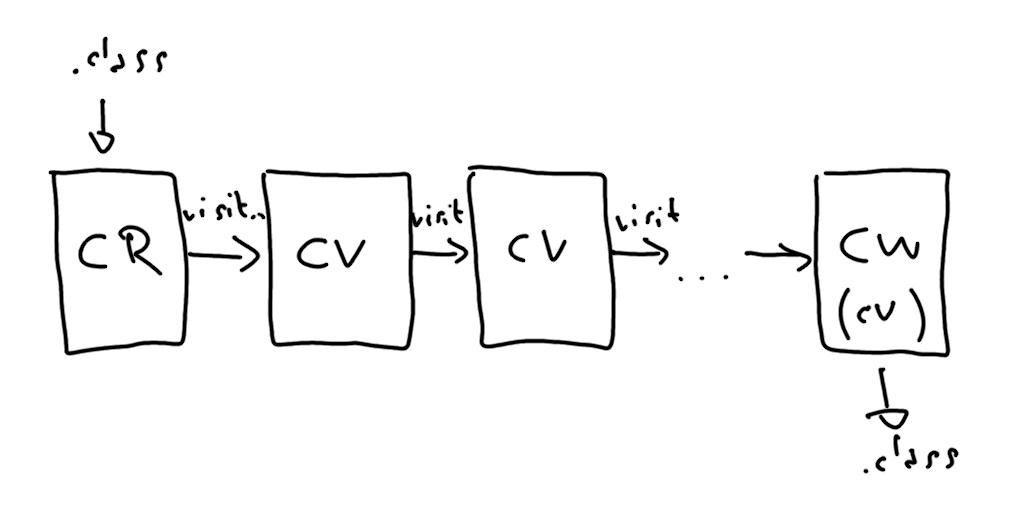
\includegraphics[width=\textwidth]{figures/asmschema.png}
    \caption{Typical architecture for class transformation. \todo{redraw}}
\end{figure}

Typical class transformation uses the following architecture: a
\texttt{ClassReader} instance reads the class, then one or more
\texttt{ClassVisitor} instances modify the class, and then a
\texttt{ClassWriter} instance writes the modified class back to a file.

\section{Dynamic Analysis using RoadRunner}

The RoadRunner framework is used for dynamic analysis of concurrent programs
written in Java. RoadRunner instruments programs to obtain a stream of events
that are useful for dynamic analysis, such as memory accesses, synchronizing on
a lock, forking or joining of threads, and so on. This event stream is then
available to various analysis tools. Multiple tools can be chained together,
each tool acting as a filter over the events. This allows complex analyses to be
built from simpler, modular tools \cite{RoadRunner}.

RoadRunner aims to simplify writing dynamic analysis tools. A RoadRunner
analysis tool only needs to handle events of interest. RoadRunner will ensure
that the event is properly detected and the event handler is called. To store
the state of the analysis, RoadRunner provides support for associating
information with memory locations, locks, or threads.

\todo{tool composition}

\todo{optional: debugging, comparing analyses}

\todo{Tool class, events, shadowThread/Var/Lock, tool composition}

\todo{instrumentation done by roadrunner}

\chapter{Contracts for Concurrency}

\todo{chapter contents}

When developing software, one frequently uses modules created by someone else
via it's programming interface. For example, in object oriented programming, the
interface consists of public methods of given class. Accessing the interface
requires one to follow a protocol consisting of: (i) syntax, i.e. types of
parameters and return values, (ii) semantics, i.e. the expected behavior for
given input parameters, and (iii) access restrictions. Access restrictions
include the domain of valid values, dependencies on other services, and
atomicity violations \cite{FITPUB11510}.

\emph{Contracts for concurrency} \cite{FITPUB10817},
\cite{DBLP:journals/corr/SousaDFL15}, are a case of a software protocol that
expresses access restrictions in concurrent setting. In its basic form, it
specifies sequences of methods that must be executed atomically. The contracts
can be extended with parameters to reflect the data flow between the methods (so
that only methods manipulating the same data must be executed atomically).
Another extension adds so called \emph{spoilers} (so that given sequence must be
executed atomically only with respect to only certain sequences). Both
extensions can be combined \cite{FITPUB11510}.


\section{Basic Contracts}

\emph{Contract} is formally defined in \cite{FITPUB10817} as follows. Let
$\Sigma_\mathbb{M}$ be a set of all public method names (the API) of a module or
a library. A \emph{contract} is a set $\mathbb{R}$ of \emph{clauses}. Each
clause $\varrho \in \mathbb{R}$ is a star-free regular expression over
$\Sigma_\mathbb{M}$. A contract violation occurs when any of the sequences in a
contract is interleaved with an execution of a method from $\Sigma_\mathbb{M}$
over the same object.

\emph{Example.} Consider a map implementation with the following operations:
\texttt{put(key, value)}, \texttt{get(key)}, \texttt{remove(key)}, and
\texttt{contains(key)}. Then a contract for this class may contain the following
clauses: \todo{formatting} \newline
    $(\varrho_1)$ \texttt{put get} \newline
    $(\varrho_2)$ \texttt{contains (put|get|remove)} \newline
Clause $\varrho_1$ states that when an element is put into the map and then
retrieved, it should be executed atomically (because the element may be removed
between the calls). Clause $\varrho_2$ states that when the program modifies the
map based on the result of the \texttt{contains} call, it should be atomic.

\todo{optional: clause composition}


\section{Parametric Contracts}

In some situations, the definition of contracts may be to restrictive, producing
false alarms. In \cite{FITPUB11510}, contracts are extended with parameters to
reflect the data flow between methods. Consider the following example:
\todo{formatting}\newline
\texttt{if (q.contains(42)) q.remove(42);} \newline
These two calls must be executed atomically only if they share the same
argument. This dependency can be expressed using \emph{meta-variables} placed as
the parameters or return values of methods. Parameters that should not be taken
into account are marked with free meta-variable (denoted with underscore).

\emph{Example.} The example from \todo{ref} can be extended with parameters:
\todo{formatting} \newline
    $(\varrho_1)$ \texttt{put(X) \_ = get(X)} \newline
    $(\varrho_2)$ \texttt{\_ = contains(X) ( put(X,\_) | \_ = get(X) | remove(X) )}
    \newline

The basic definition of contracts in fact contains one implicit parameter, the
object that the method was called upon (\texttt{this} in Java)
\cite{FITPUB10817}. To better illustrate this, the example can be rewritten as:
\todo{formatting} \newline
    $(\varrho_1)$ \texttt{X.put(Y) \_ = X.get(Y)} \newline
    $(\varrho_2)$ \texttt{\_ = X.contains(Y) ( X.put(Y,\_) | \_ = X.get(Y) | X.remove(Y) )}


\section{Contracts with Spoilers}

In \cite{FITPUB11510}, contracts are extended with contextual information to
distinguish which method sequences violates the contract. Each clause of the
basic contract is called a \emph{target}, and is assigned a set of so called
\emph{spoilers}. A spoiler is a set of method sequences that may violate its
target.

Consider the clause $\varrho_1$ from example \todo{ref example in Basic
Contracts}. If the element that was put to the map is concurrently removed or
updated before the \texttt{get} call, a contract violation should be detected.
However, calling \texttt{contains} or \texttt{get} on the element will not
affect the computation and should not be marked as a contract violation. In this
example, sequences \texttt{put} and \texttt{remove} are spoilers for a target
 $\varrho_1$, denoted as \texttt{put get} $\leftsquigarrow$
\texttt{put|remove}.

% TODO: this is basically copied - is it ok?

Formally, as defined in \cite{FITPUB11510}, let $\mathbb{R}$ be the set of
\emph{target} clauses where each target $\varrho \in \mathbb{R}$ is a regular
expression over $\Sigma_\mathbb{M}$. Let $\mathbb{S}$ be the set of
\emph{spoilers} where each spoiler $\sigma \in \mathbb{S}$ is a regular
expression over $\Sigma_\mathbb{M}$. A \emph{contract} is a relation $\mathbb{C}
\subseteq \mathbb{R} \times \mathbb{S}$ defining for each target, which spoilers
may cause atomicity violation.

Contract violation is observed when a target sequence $\varrho \in \mathbb{R}$
is fully interleaved by a spoiler sequence $\sigma \in \mathbb{C}(\varrho)$, and
the sequences are executed on the same object.

\emph{Example.} The example from \todo{ref} can be extended with spoilers:
\todo{formatting} \newline
    $(\varrho_1)$ \texttt{put get} $\leftsquigarrow$ \texttt{put|remove} \newline
    $(\varrho_2)$ \texttt{contains (put|get|remove)} $\leftsquigarrow$
    \texttt{put|remove} \newline

\todo{combining spoilers and parameters}


\section{Dynamic Contract Validation}

\todo{section intro}

\subsection{Multi-threaded Program Traces}

For the purposes of dynamic contract validation, multi-threaded program
\emph{trace} consists of events of the following types:
\begin{itemize}
    \item thread forking or joining another thread,
    \item thread entering or exiting a method,
    \item thread acquiring or releasing a lock.
\end{itemize}

All events in a trace are indexed by their position in the trace. Let
$\mathbb{T}$ be a set of threads, $\mathbb{R}$ a set of targets, $\mathbb{S}$ a
set of spoilers, $\mathbb{C} \subseteq \mathbb{R} \times \mathbb{S}$ a set of
contracts, and $\mathbb{L}$ a set of locks. The set of all events that can be
generated by a thread $t \in \mathbb{T}$ is then denoted as $\mathbb{E}_t$. Let
$\mathbb{E} = \bigcup_{t \in \mathbb{T}} \mathbb{E}_t$. A \emph{trace} is then a
sequence $\tau = e_1 \hdots e_n \in \mathbb{E}^+$.

% TODO: basically copied

Given a trace $\tau = e_1 \hdots e_n \in \mathbb{E}^+$, we call its subsequence
$r = e_{i_1} e_{i_2} \hdots e_{i_k}$, $1 < k \leq n$, an \emph{instance} of a
target $\varrho \in \mathbb{R}$ if, and only if:
\begin{itemize}
    \item \todo{}
\end{itemize}

\todo{}

\todo{ \newline
    * trace windows \newline
    * discarding spoilers and targets \newline
    * main algorithm \newline
    * optimizations, vector clocks, happens-before \newline
}



\chapter{Design of a Dynamic Analyzer for Parametric Contracts with Spoilers}

\todo{ \newline
    * design of a RoadRunner tool \newline
    * requirements \newline
    * required changes to RR internals \newline
    * contract limitation? \newline
}



\chapter{Implementation of a Contract Validator for RoadRunner}

\todo{}



\chapter{Evaluation}

\todo{}



\chapter{Conclusion}

\todo{}
